\chapter{結果と評価}
\label{chap:results}
本章では,3章で紹介した手法によって自動生成した吹奏アニメーションについて記述する.
\secref{sec:system}では仕様したPCやシステムの仕様を述べ,
\secref{sec:result}では自動生成した吹奏アニメーションのキャプチャリング画像を示す.
そして\secref{sec:review}では自動生成結果を実際の演奏シーンや既存の吹奏アニメーションと比較することにより,提案手法を評価する.

\section{実行環境} \label{sec:system}
事前にUnreal Engineにて専用のプロジェクトを作成し,モーションのデータが記載されているUnreal Engine専用のファイルをインポートする.
そして,キャラクタと,それぞれが演奏する楽器を\figref{fig:ue4}のようにセッティングする.
なお,最初にインポートするUnreal Engine専用のファイルには,キャラクタの姿勢データも存在するため,
キャラクタの姿勢のセッティングは容易にできる.\\
\indent
実行環境は\tabref{tab:pc}の通りである.
\begin{figure}[h]
	\centering
	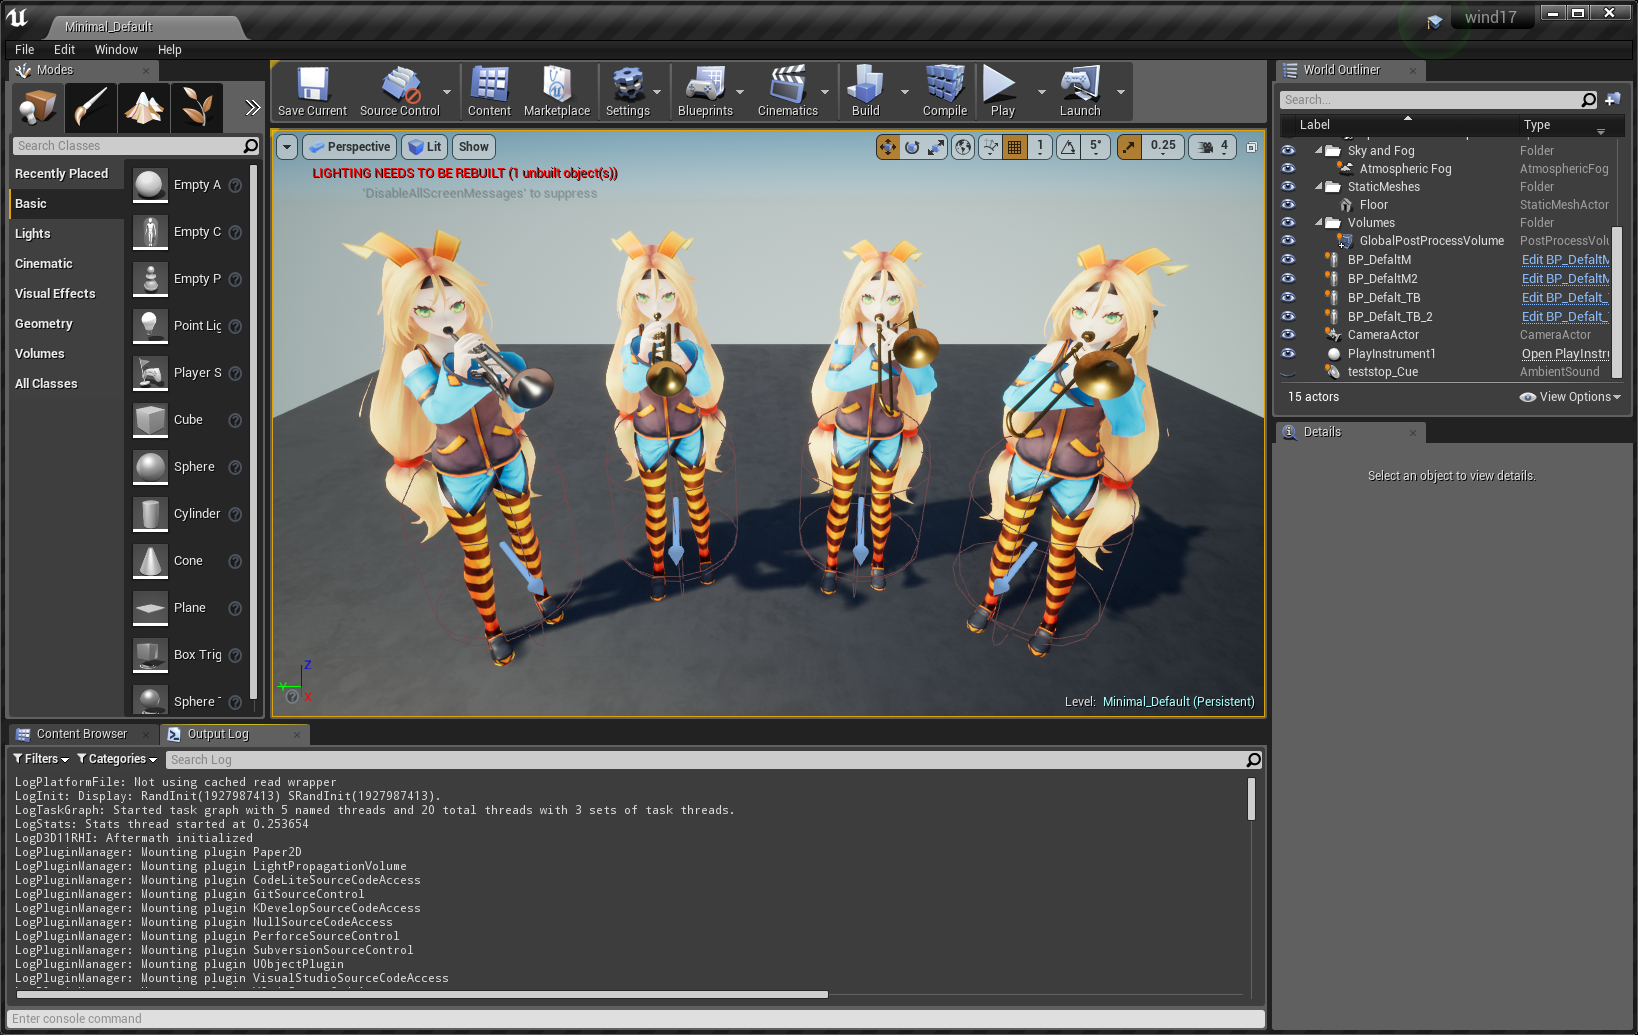
\includegraphics[width=14cm]{fig/chap4/ue4.eps}
	\caption{Unreal Engineの初期設定}
	\label{fig:ue4}
\end{figure}

\begin{table}[htbp] 
	\begin{center}
		\caption{実行環境}
		\label{tab:pc}
		\begin{tabular}{|l|c|}
			\hline
			OS & Windows10 64bit \\ \hline
			CPU & Intel\textregistered Core\textsuperscript{TM}i7-3930K \\ \hline
			RAM & 32.00GB\\ \hline
			言語 & c++\\ \hline
		\end{tabular}
	\end{center}
\end{table}

\section{アニメーション生成結果} \label{sec:result}
本研究で作成したアニメーションは,主に少人数編成であるアンサンブルアニメーションである.
以下では,トランペット奏者2名で演奏するアニメーションのキャプチャリング画像と,
トランペット奏者2名,トロンボーン奏者2名の計4名で演奏するアニメーションのキャプチャリング画像を示す.
以下,それぞれについて制御している口元やボーンの制御について説明するが,
前者のアニメーションは,トランペット奏者の口元や指元がズームインされているシーンであるため,主に口元や指元のボーンの制御について,
後者のアニメーションは全体を俯瞰しているシーンであるため,前者のアニメーションにて述べなかったボーンの制御について記述する.\\
\indent
\figref{anim1}は,トランペット奏者2名の基本姿勢である.
\begin{figure}[h]
	\centering
	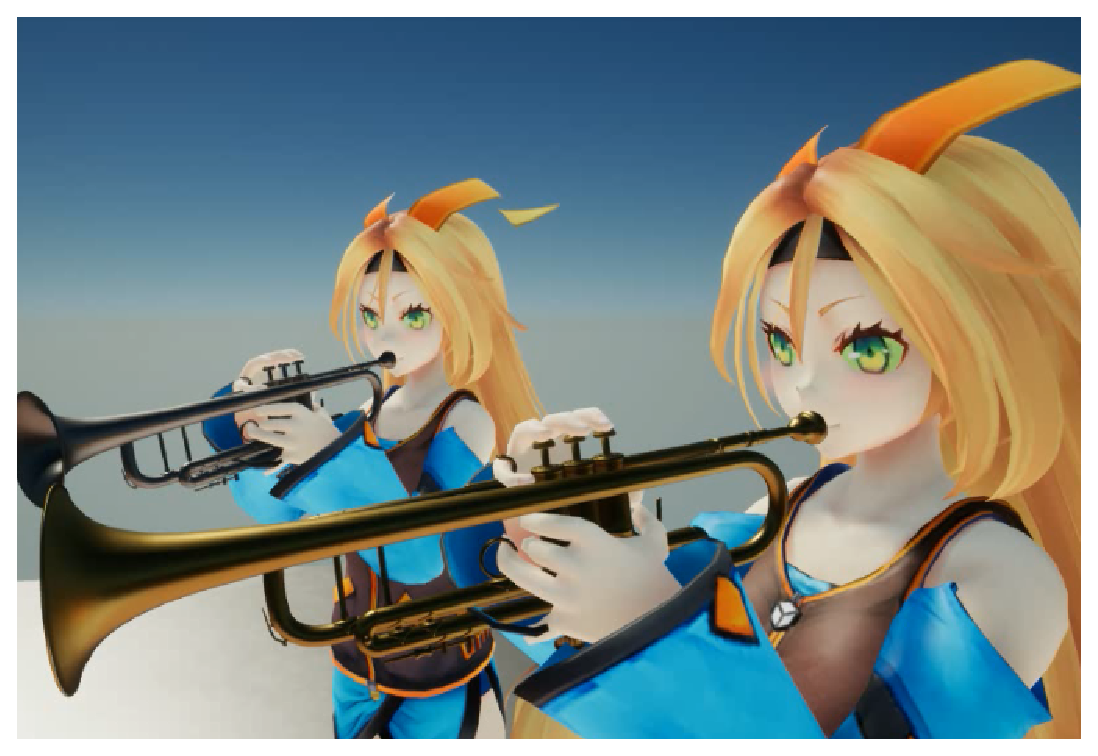
\includegraphics[width=10cm]{fig/chap4/anim1.eps}
	\caption{トランペット奏者2名の基本姿勢}
	\label{fig:anim1}
\end{figure}
トランペット奏者は,\figref{anim1_finger}のように指でトランペットのピストンを押す.
\begin{figure}[h]
	\centering
	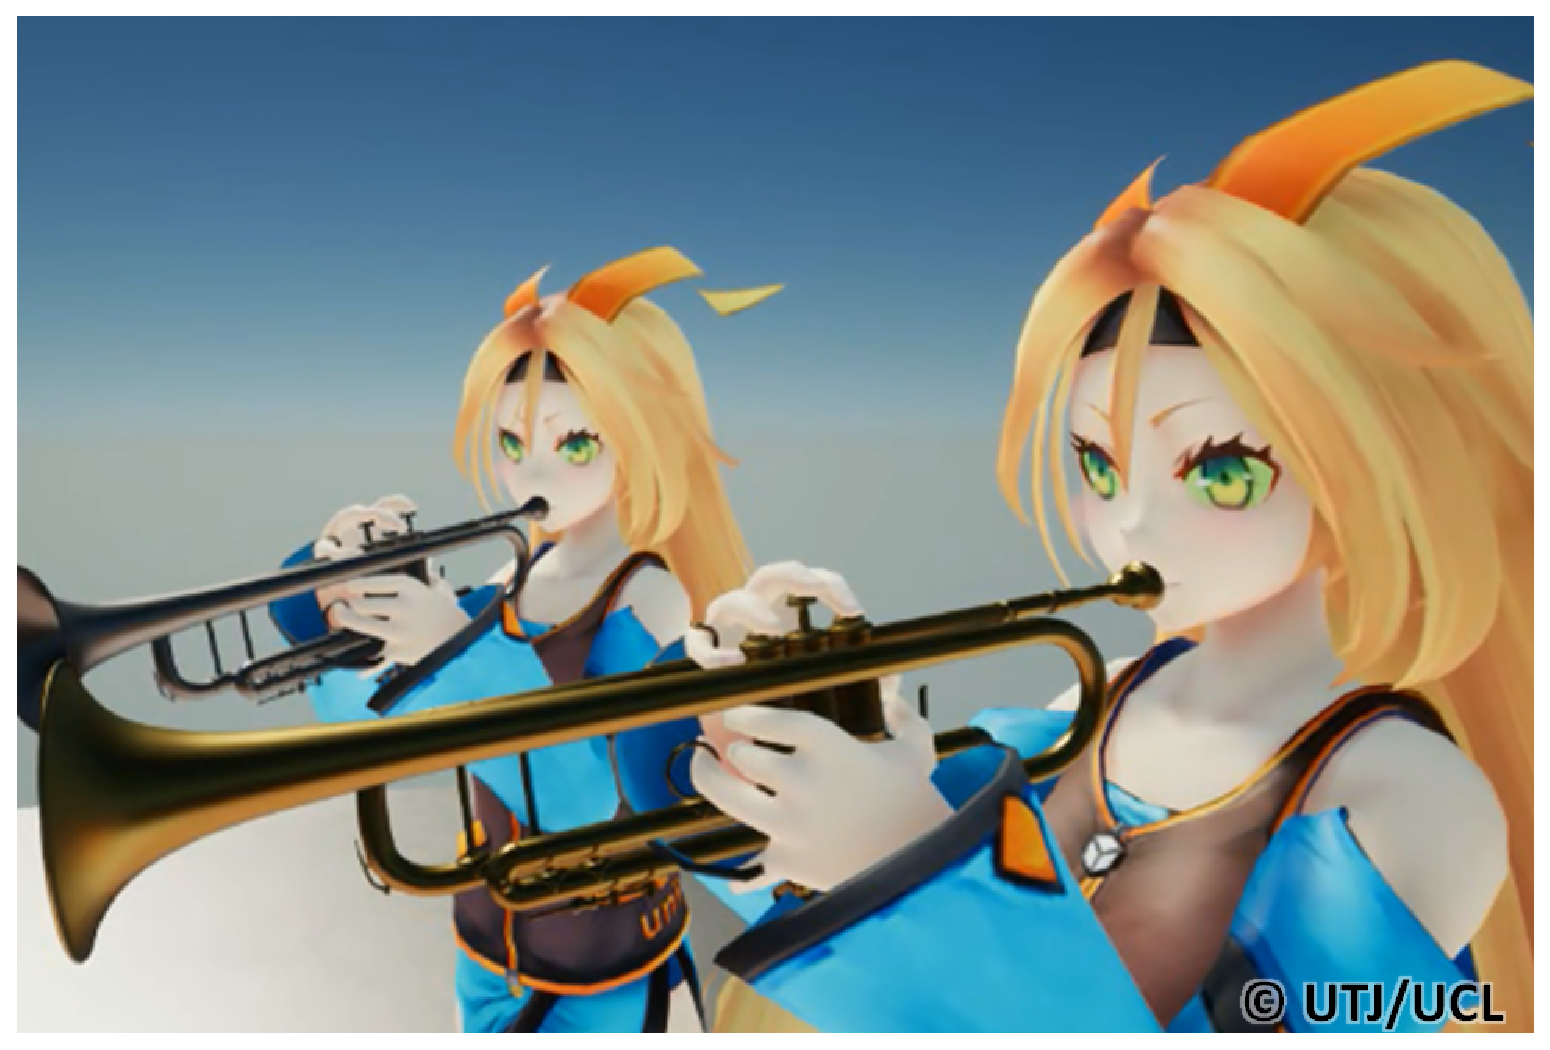
\includegraphics[width=10cm]{fig/chap4/anim1_finger.eps}
	\caption{トランペット奏者がピストンを押す様子}
	\label{fig:anim1_finger}
\end{figure}
息継ぎをするタイミングでは,演奏者は\subfigref{fig:zoom}{fig:breath}のように口を開ける.
また,高音を演奏するタイミングでは,\subfigref{fig:zoom}{fig:high}のように口元が緊張する.
\begin{figure}[t]
	\centering
	\subcaptionbox{\textgt{通常の口元の様子}
		\label{fig:default}}[0.75\linewidth]{
		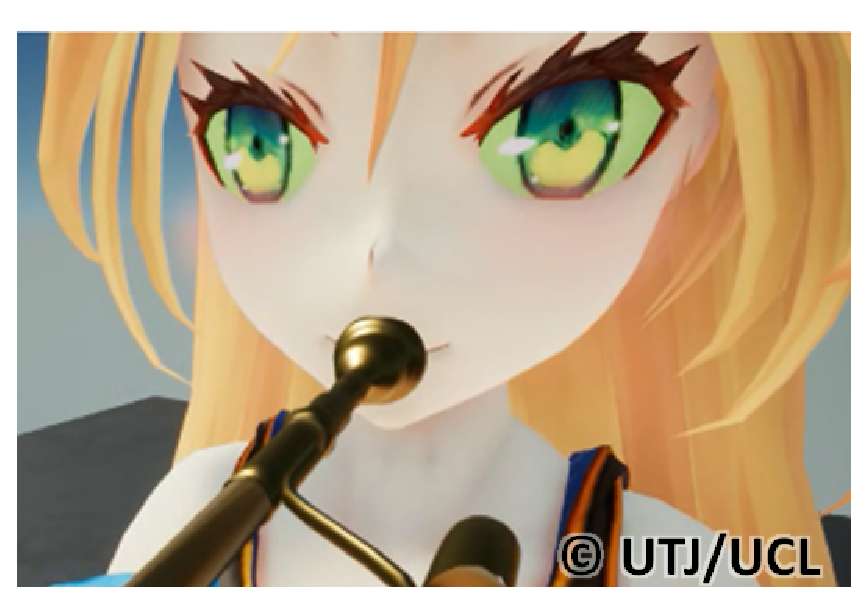
\includegraphics[height=5.5cm]{fig/chap4/anim1_zoom.eps}}
	\subcaptionbox{\textgt{息継ぎをしている様子}
		\label{fig:breath}}[0.6\linewidth]{
		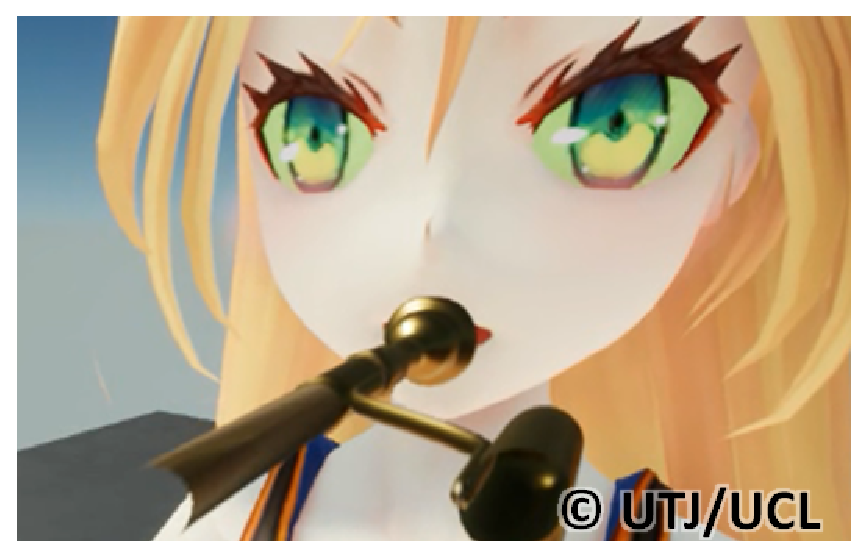
\includegraphics[height=5.5cm]{fig/chap4/anim1_zoom_breath.eps}}
	\subcaptionbox{\textgt{高い音を演奏し口元が緊張している様子}
		\label{fig:high}}[0.6\linewidth]{
		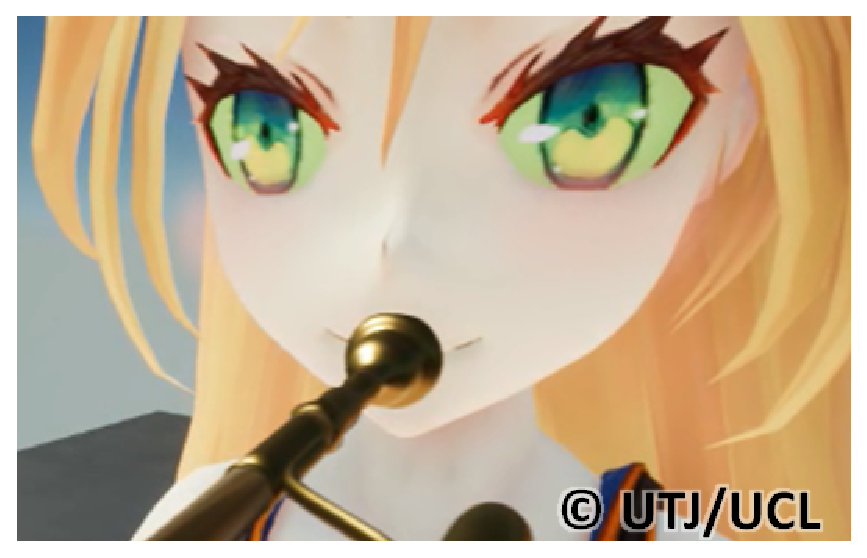
\includegraphics[height=5.5cm]{fig/chap4/anim1_zoom_high.eps}}
	\caption{演奏者の口元}
	\label{fig:zoom}
\end{figure}
\figref{anim2}は,トランペット奏者2名,トロンボーン奏者2名の基本姿勢である.
\begin{figure}[h]
	\centering
	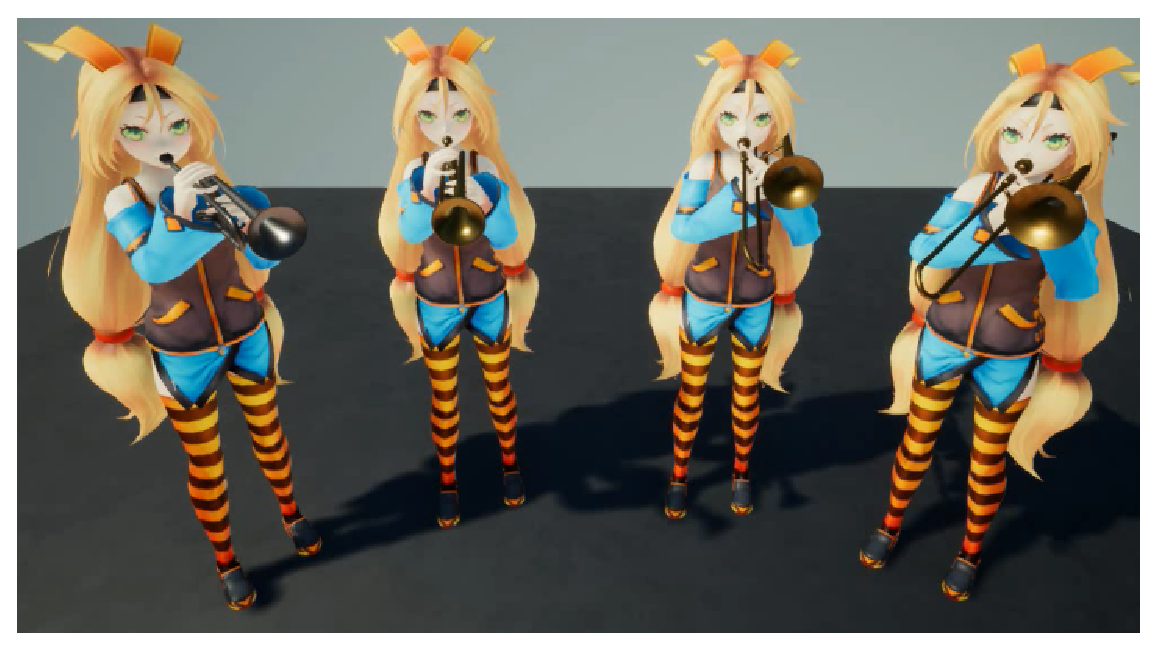
\includegraphics[width=10cm]{fig/chap4/anim2.eps}
	\caption{トランペット奏者2名とトロンボーン奏者2名の基本姿勢}
	\label{fig:anim2}
\end{figure}
トロンボーン奏者は,\figref{anim2_zoom}のように右手でスライドを動かす.
\begin{figure}[h]
	\centering
	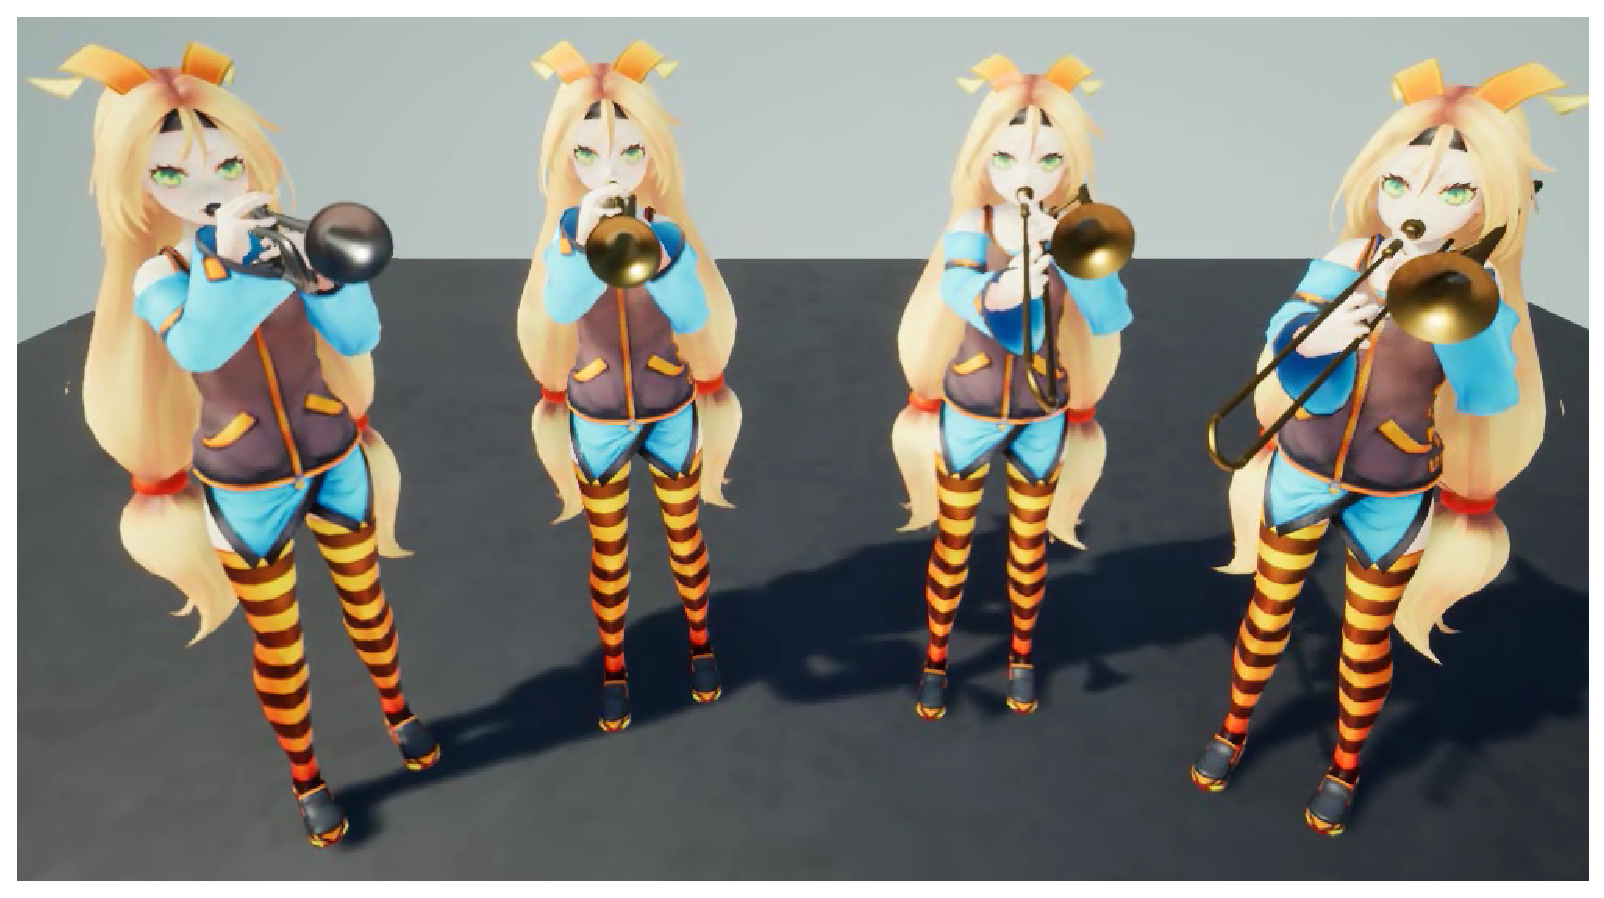
\includegraphics[width=10cm]{fig/chap4/anim2_slide.eps}
	\caption{トロンボーン奏者がピストンを動かす様子}
	\label{fig:anim2_zoom}
\end{figure}
曲の入りでは,タイミングを合わせるために,膝を使って楽器を縦に振る.
\figref{anim2_down}は,膝を曲げ,楽器を下に向けた瞬間の様子である.
\begin{figure}[h]
	\centering
	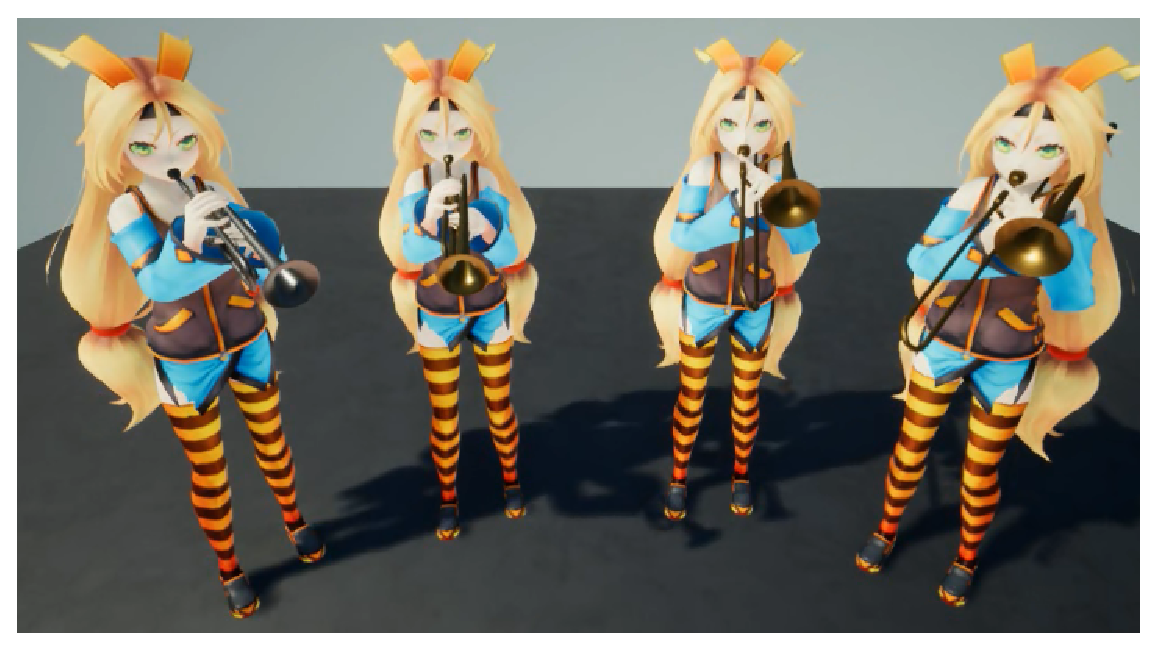
\includegraphics[width=10cm]{fig/chap4/anim2_down.eps}
	\caption{曲の入りを合わせるために膝を使い楽器を下に向けた瞬間の様子}
	\label{fig:anim2_down}
\end{figure}
息継ぎをするタイミングでは,演奏者は身体を反らす.
\figref{anim2_breath}のは,トランペット奏者2名が息継ぎをしている瞬間の様子である.
\begin{figure}[h]
	\centering
	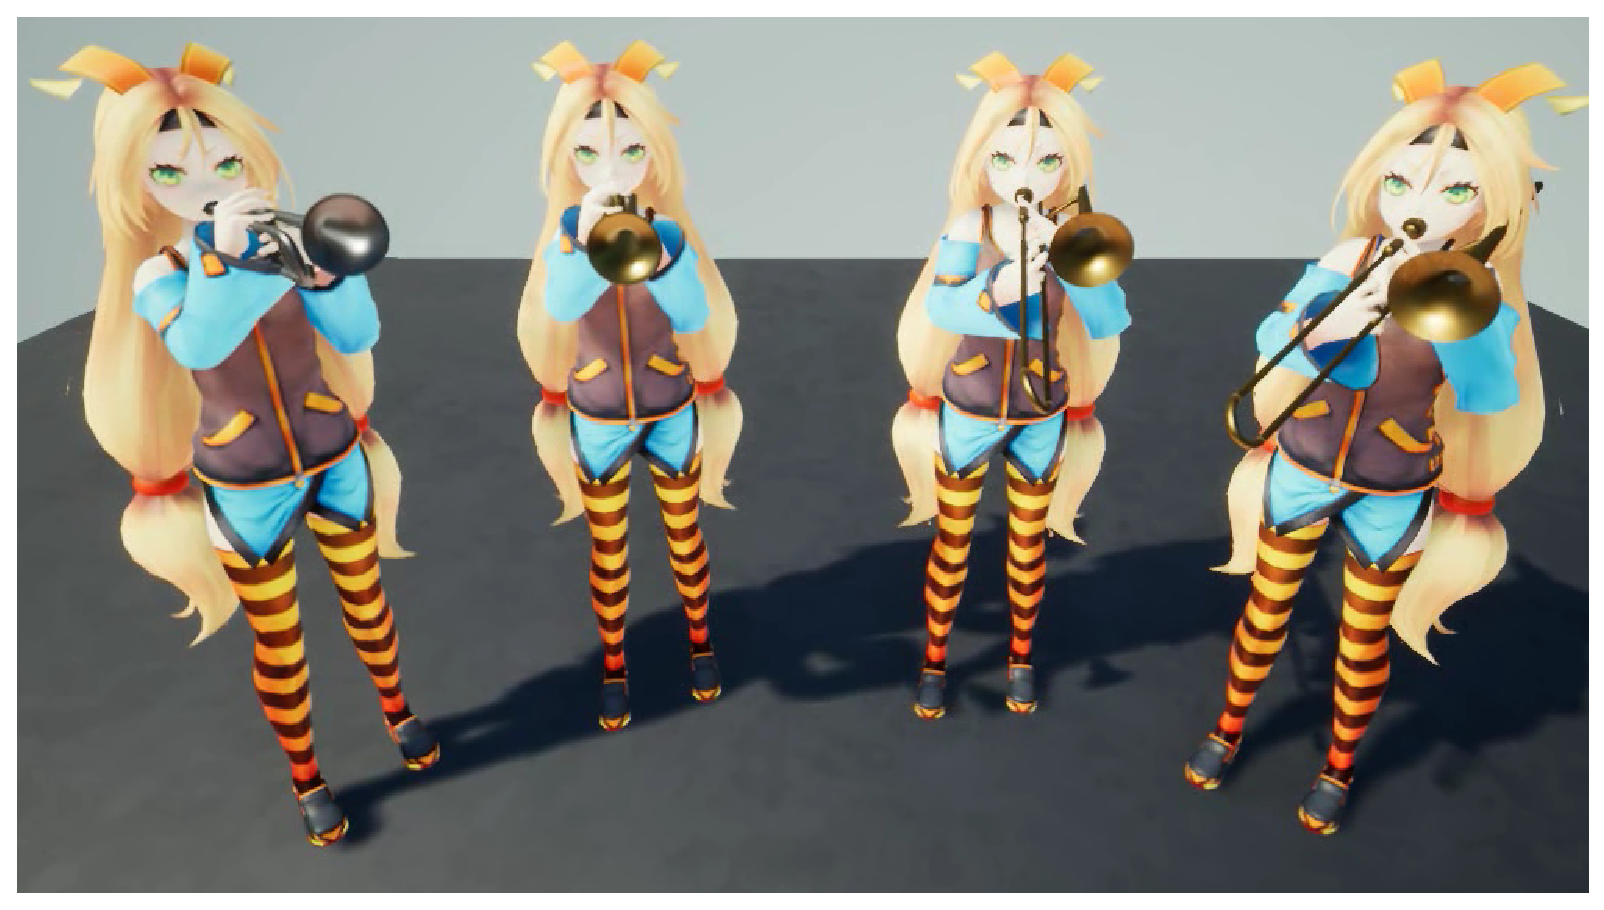
\includegraphics[width=10cm]{fig/chap4/anim2_breath.eps}
	\caption{息継ぎしている瞬間の様子}
	\label{fig:anim2_breath}
\end{figure}

\section{評価} \label{sec:review}
自動生成した吹奏アニメーションに対して,以下の3つの評価を行った.
\begin{itemize}
	\item 実際の演奏シーンとの比較による評価
	\item 既存のアニメーションとの比較による評価
	\item アンサンブルアニメーションの評価
\end{itemize}
以下,評価結果を,吹奏楽やオーケストラ経験者,吹奏楽やオーケストラ未経験者に分けて示す.

\subsection{実際の演奏シーンとの比較による評価}
トランペット奏者やトロンボーン奏者が実際に演奏しているシーンと,自動生成した吹奏アニメーションを比較してもらい,以下の2項目についてアンケートをとった.
\begin{itemize}
	\item 指や腕の動きは再現できているか
	\item 演奏している雰囲気はあるか
\end{itemize}
その結果をに示す.
\begin{figure}[t]
	\centering
	\subcaptionbox{\textgt{吹奏楽・オーケストラ経験者の回答}
		\label{fig:unity}}{
		\includegraphics[width=6cm]{fig/chap4/Q1_tp1.eps}}
	\hspace{2mm}
	\subcaptionbox{\textgt{吹奏楽・オーケストラ未経験者の回答}
		\label{fig:tp}}{
		\includegraphics[width=6cm]{fig/chap4/Q1_tp2.eps}}
	\caption{トランペット奏者の指の動きは再現できているか}
	\label{fig:Q1-tp}
\end{figure}

\begin{figure}[t]
	\centering
	\subcaptionbox{\textgt{吹奏楽・オーケストラ経験者の回答}
		\label{fig:unity}}{
		\includegraphics[width=7cm]{fig/chap4/Q1_tb1.eps}}
	\subcaptionbox{\textgt{吹奏楽・オーケストラ未経験者の回答}
		\label{fig:tp}}{
		\includegraphics[width=7cm]{fig/chap4/Q1_tb2.eps}}
	\caption{演奏アニメーションが不自然であると感じることがあるかどうか}
	\label{fig:Q1-tb}
\end{figure}

\subsection{既存のアニメーションとの比較による評価}
既存の吹奏アニメーションにおける,トランペット奏者やトロンボーン奏者が実際に演奏しているシーンと,自動生成した吹奏アニメーションを比較してもらい,以下の2項目についてアンケートをとった.
\begin{itemize}
	\item 指や腕の動きは,どちらの方が音楽のリズムに合っているか
	\item 自動生成した吹奏アニメーションの,キャラクタの身体の動きは自然か
\end{itemize}
その結果を\figref{fig:Q2-tp}に示す.
\begin{figure}[t]
	\centering
	\subcaptionbox{\textgt{吹奏楽・オーケストラ経験者の回答}
		\label{fig:unity}}{
		\includegraphics[width=6cm]{fig/chap4/Q1_tp1.eps}}
	\hspace{2mm}
	\subcaptionbox{\textgt{吹奏楽・オーケストラ未経験者の回答}
		\label{fig:tp}}{
		\includegraphics[width=6cm]{fig/chap4/Q1_tp2.eps}}
	\caption{指や腕の動きは,どちらの方が音楽のリズムに合っているか}
	\label{fig:Q2-tp}
\end{figure}

\begin{figure}[t]
	\centering
	\subcaptionbox{\textgt{吹奏楽・オーケストラ経験者の回答}
		\label{fig:unity}}{
		\includegraphics[width=7cm]{fig/chap4/Q1_tb1.eps}}
	\subcaptionbox{\textgt{吹奏楽・オーケストラ未経験者の回答}
		\label{fig:tp}}{
		\includegraphics[width=7cm]{fig/chap4/Q1_tb2.eps}}
	\caption{自動生成した吹奏アニメーションの,キャラクタの身体の動きは自然か}
	\label{fig:Q2-tb}
\end{figure}

\subsection{アンサンブルアニメーションの評価}
既存の吹奏アニメーションにおける,トランペット奏者やトロンボーン奏者が実際に演奏しているシーンと,自動生成した吹奏アニメーションを比較してもらい,以下の2項目についてアンケートをとった.
\begin{itemize}
	\item 指や腕の動きは,どちらの方が音楽のリズムに合っているか
	\item 自動生成した吹奏アニメーションの,キャラクタの身体の動きは自然か
\end{itemize}
その結果を\figref{fig:Q2-tp}に示す.
\begin{figure}[t]
	\centering
	\subcaptionbox{\textgt{吹奏楽・オーケストラ経験者の回答}
		\label{fig:unity}}{
		\includegraphics[width=6cm]{fig/chap4/Q1_tp1.eps}}
	\hspace{2mm}
	\subcaptionbox{\textgt{吹奏楽・オーケストラ未経験者の回答}
		\label{fig:tp}}{
		\includegraphics[width=6cm]{fig/chap4/Q1_tp2.eps}}
	\caption{指や腕の動きは,どちらの方が音楽のリズムに合っているか}
	\label{fig:Q2-tp}
\end{figure}

\begin{figure}[t]
	\centering
	\subcaptionbox{\textgt{吹奏楽・オーケストラ経験者の回答}
		\label{fig:unity}}{
		\includegraphics[width=7cm]{fig/chap4/Q1_tb1.eps}}
	\subcaptionbox{\textgt{吹奏楽・オーケストラ未経験者の回答}
		\label{fig:tp}}{
		\includegraphics[width=7cm]{fig/chap4/Q1_tb2.eps}}
	\caption{自動生成した吹奏アニメーションの,キャラクタの身体の動きは自然か}
	\label{fig:Q2-tb}
\end{figure}

\subsection{システムの有用性の予想}
アニメーション制作に関する知識がある者に,本手法によりアニメーション制作の労力や時間が軽減されると思うか否かを質問した.
その結果,のような結果を得た.